\documentclass[12pt]{article}

\usepackage[utf8]{inputenc}
\usepackage{color}
\usepackage{graphicx}

\title{Manual Básico de LaTeX}
\author{
	Elyas Correa Nogueira\\
	\and
	Fabiana Silva Finoti\\
	\and
	Isabela Daiana Pereira\\
	\and
	Israel Mateus Melo Oliveira\\	
}
\date{6 de Maio de 2019}

\begin{document}
	
	\maketitle
	
	\newpage
	
	\section{Introdução}
		O Latex (estilizado como \LaTeX) é um sistema de preparação de documentos desenvolvido nos anos 80 pelo americano Leslie Lamport. Amplamente empregado na fabricação de documentos, o LaTeX utiliza texto simples para a confecção dos arquivos, fazendo a formatação do texto (\textit{itálico}, \textbf{negrito} {\color{red} cores}) por meio de marcadores, de maneira que o escritor foque no conteúdo ao invés da estilização.
	
		A padronização dos documentos oferecidos pelo LaTeX faz com que ele seja preferencial na fabricação de vários documentos acadêmicos, eliminando assim erros na formatação de tais documentos. Neste manual, será abordada a estrutura básica de um documento TeX e vários pacotes que oferecem funcionalidades importantes para quem está escrevendo o documento.
	
	\section{Como utilizar o LaTeX?}
	
		\subsection{Instalação em Linux e Windows}
		
			\subsubsection{Instalação em Ubuntu}
				Para facilitar o processo, será explicado como instalar o LaTeX em um sistema Ubuntu. Abra o terminal e digite a seguinte linha:\\\\
				\texttt{sudo apt-get install texlive texlive-latex-extra texlive-lang-portuguese}\\
			
				Assim, será instalado em seu computador os pacotes necessários para compilar arquivos básicos .tex. Para o uso de ferramentas mais complexas, pode ser necessária a instalação de outros pacotes -- como o \texttt{texlive-math-extra}, usado para matemática complexa. 
			
				Uma vez que os pacotes de compilação foram instalados, você precisará de um editor para começar a sua aventura LaTeX. Para respeitar o que foi utilizado em aula, é recomendado que você use o TeXstudio. Para instalá-lo, abra o terminal e digite:\\\\
				\texttt{sudo apt-get install texstudio}
			
			\subsubsection{Instalação em Windows}
				No Windows, a instalação dos compiladores e do editor podem ser feitas por meio do browser. Entre no link \texttt{https://miktex.org/download}, tenha certeza que você está na aba do Windows e clique no botão de Download (o site oferece um tutorial passo-a-passo em caso de dúvidas). Quando o arquivo for baixado, abra o instalador, faça bom uso do 'Avançar' e espere o fim do processo.
			
				Agora que os compiladores estão instalados, chegou a hora do editor. Entre no link \texttt{http://texstudio.sourceforge.net/}, clique na aba de Downloads, ache a versão correspondente ao seu Windows e espere o fim do download. Abra o instalador e vá clicando em 'Avançar' até que o TeXstudio esteja instalado em seu computador.
			
		\subsection{Criação de Documento Básico}
			Nessa subseção, você será apresentado a um código básico de LaTeX e as linhas serão explicadas posteriormente.
			
			\begin{figure}[h]
				\begin{center}
					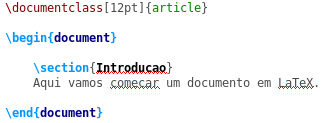
\includegraphics{codigo1.png}
				\end{center}
			\end{figure}
		
			Na primeira linha, o escritor declara que o documento digitado será do tipo \textit{article}, ou seja, seguirá os padrões de formatação de um artigo acadêmico, com \texttt{12pt} sendo o tamanho da fonte utilizada.
			A linha seguinte aponta que o documento começará a ser escrito, abrindo assim um bloco que contém todas as informações que serão utilizadas.
		    
			O LaTeX organiza os tópicos em seções. Sendo assim, o usuário consegue distribuir todos as seções do documento desejado utilizando o marcador da imagem.
		    
		    
		\subsection{Estrutura de Documento}
		
		\subsection{Matemática}
		
		\subsection{Imagens}
		
		\subsection{Tabela de Conteúdos}
		
		\subsection{Bibliografia}
		
		\subsection{Notas de Rodapé}
			Uma nota de rodapé pode ser inserida após a palavra ou frase a qual se refere através do comando:
			\begin{figure}[h]
				\centering
				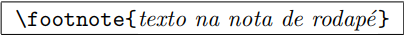
\includegraphics[scale=0.5]{no.png}
			\end{figure}
			
			O número é opcional, e pode ser usado para forçar um determinado numero ao invés do automático que seria gerado pelo compilador o texto é o que vai aparecer na nota no final da página.\\
			Exemplo:
			\begin{figure}[h]
				\centering
				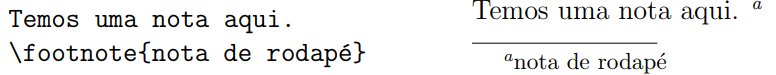
\includegraphics[scale=0.45]{xx.png}
			\end{figure}
		
		\subsection{Tabelas}
		
				\subsubsection{Tabular}
					Uma tabela pode ser especificada pelo ambiente tabular. É possível utilizar linhas horizontais e verticais sem se preocupar com a largura das colunas que é calculada automaticamente pelo LATEX. A criação de uma tabela é feita da seguinte forma:
					\begin{figure}[h]
						\centering
						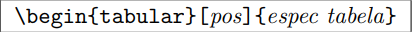
\includegraphics[scale=0.45]{t.png}
					\end{figure}
		
					O argumento \textit{espec} especifica a quantidade e alinhamentos das colunas:
					\begin{itemize}
						\item \textbf{$|$}: adiciona uma linha vertical;
						\item \textbf{l}: indica uma coluna alinhada `a esquerda;
						\item \textbf{r}: indica uma coluna alinhada `a direita;
						\item \textbf{c}: indica uma coluna com texto centralizado;
						\item \textbf{p\{{largura}\}}: indica uma coluna especial com texto justificado capaz de quebrar linhas, com a largura especificada com unidade de medida.
					\end{itemize}
					Para mesclar colunas de células podemos usar o comando\\
					$\backslash$multicolumn\{{num}\}\{{formato}\}{\{texto}\}
					que concatena o número de colunas especificado por \textit{num} com o alinhamento especificado por \textit{formato} e possui como conteúdo \textit{texto}.\\ 
					Uma tabela pode ser inserida dentro do ambiente \textit{table} o que faz dela um objeto flutuante. Vantagens de utilizar esse tipo de ambiente é a posição correta da tabela no texto, sem que seja quebrada em das páginas, por exemplo, faz com que a tabela apareça em um índice de tabelas e também a inserção de rótulos e legendas.
					O argumento \textit{pos} especifica a posição vertical da tabela relativamente à linha base do texto envolvente. Use as letras \textit{t}, \textit{b}, \textit{c} e \textit{p} para especificar o alinhamento da tabela no topo, fundo, centro ou em uma página especial contendo somente objetos flutuantes respectivamente. \textit{!} é usado para  ignora alguns parâmetros internos.\\
					Dentro de um ambiente tabular, o \& salta para a próxima coluna, $\backslash$$\backslash$
					inicia uma nova linha e $\backslash$hline insere uma linha horizontal. Pode adicionar
					linhas parciais usando $\backslash$cline{j-i}, onde j e i são os números das colunas
					de onde e para onde a linha se deve estender.
					\\
					A seguir apresentamos uma tabela criada como objeto flutuante:
					\begin{table}[ht]
						\begin{center}
							\begin{tabular}{|c|r|l|}
								\hline
								Centro & Direita & Esquerda \\
								\hline
								\hline
								\multicolumn{3}{|c|}{Números}\\
								\hline
								1 & 2 & 3 \\ \cline{2-3}
								4 & 5 & 6 \\
								\hline
							\end{tabular}
							\caption{Uma tabela simples}
						\end{center}
					\end{table}
		
		
		
					Agora, apresentamos os códigos utilizados para gerar a Tabela 1 mostrada:\\
					\texttt{$\backslash$begin\{{table}\}[ht]\\}
					\texttt{$\backslash$begin\{{center}\}\\}
					\texttt{$\backslash$begin\{{tabular}\}{\{$|$c$|$r$|$l$|$}\}\\}
					\texttt{$\backslash$hline\\}
					\texttt{Centro \& Direita \& Esquerda \\}
					\texttt{$\backslash$hline \\}
					\texttt{$\backslash$hline\\}
					\texttt{$\backslash$multicolumn\{{3}\}{\{$|$c$|$}\}{\{Números}\}\\}
					\texttt{$\backslash$hline \\}
					\texttt{1 \& 2 \& 3 $\backslash$$\backslash$ $\backslash$cline\{{2-3}\}\\
						4 \& 5 \& 6 \\}
					\texttt{$\backslash$hline \\}
					\texttt{$\backslash$end\{{tabular}\}\\}
					\texttt{$\backslash$caption\{{Uma tabela simples}\}\\}
					\texttt{$\backslash$end\{{center}\}\\}
					\texttt{$\backslash$end\{{table}\}\\}
		
					Para mesclar facilmente as linhas das células podemos usar o pacote
					\textit{multirow} que possui o comando $\backslash$multirow que funciona de maneira análoga
					ao $\backslash$multicolumn, sendo que é possível passar como posição um *, indicando
					que o compilador deve procurar pelo melhor ajuste, e é preciso deixar a posição correspondente da coluna cujas linhas estão sendo mescladas em branco.\\
					Um pequeno exemplo:\\
		
					\begin{center}
						\begin{tabular}{|c|r|r|l|}
							\hline
							Centro & Direita & Direita & Esquerda \\
							\hline
				
							& 4 & 5 & 6 \\
							\hline
						\end{tabular}
					\end{center}
					O código do exemplo mostrado:\\
					\texttt{$\backslash$begin\{{tabular}\}\{{$|$c$|$r$|$r$|$l$|$}\}\\}
					\texttt{$\backslash$hline \\}
					\texttt{Centro \& Direita \& Direita \& Esquerda \\}
					\texttt{$\backslash$hline\\}
					\texttt{$\backslash$multirow\{{2}\}\{{*}\}\{{Números}\} \& 1 \& 2 \& 3 \\}
					\texttt{\& 4 \& 5 \& 6 \\}
					\texttt{$\backslash$hline}
					\texttt{$\backslash$end\{{tabular}\}}
		
				\subsubsection{Table}	
		
					O ambiente \textit{table} possibilita a inclusão de uma legenda para a tabela e trabalha a mesma como um objeto flutuante. A sintaxe deste ambiente é
		
					\begin{figure}[h]
						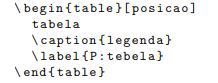
\includegraphics[scale=0.7]{a.png}
					\end{figure}
					Onde posição é o parâmetro que indica onde a tabela deve ser preferencialmente inserida, tabela corresponde ao código da tabela a ser inserida, $\backslash$caption é o comando correspondente a legenda e legenda é o texto a ser apresentado como legenda, $\backslash$label é o comando para referência cruzada como já apresentado.
					Exemplo contendo uma tabela e o código correspondente:
					\begin{figure}[h]
						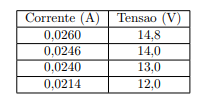
\includegraphics[scale=0.7]{q.png}
					\end{figure}
					\begin{figure}[h]
						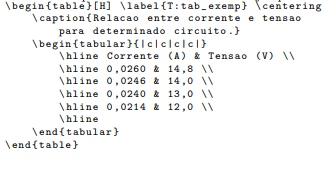
\includegraphics[scale=0.7]{qq.png}
					\end{figure}
		
		\subsection{Geração automática de Tabelas}
			Para se gerar uma tabela automaticamente, basta visitar o site \texttt{http://tablesgenerator.com/}. Este site, possui a seguinte interface:
			
			\begin{figure}[h]
				\centering
				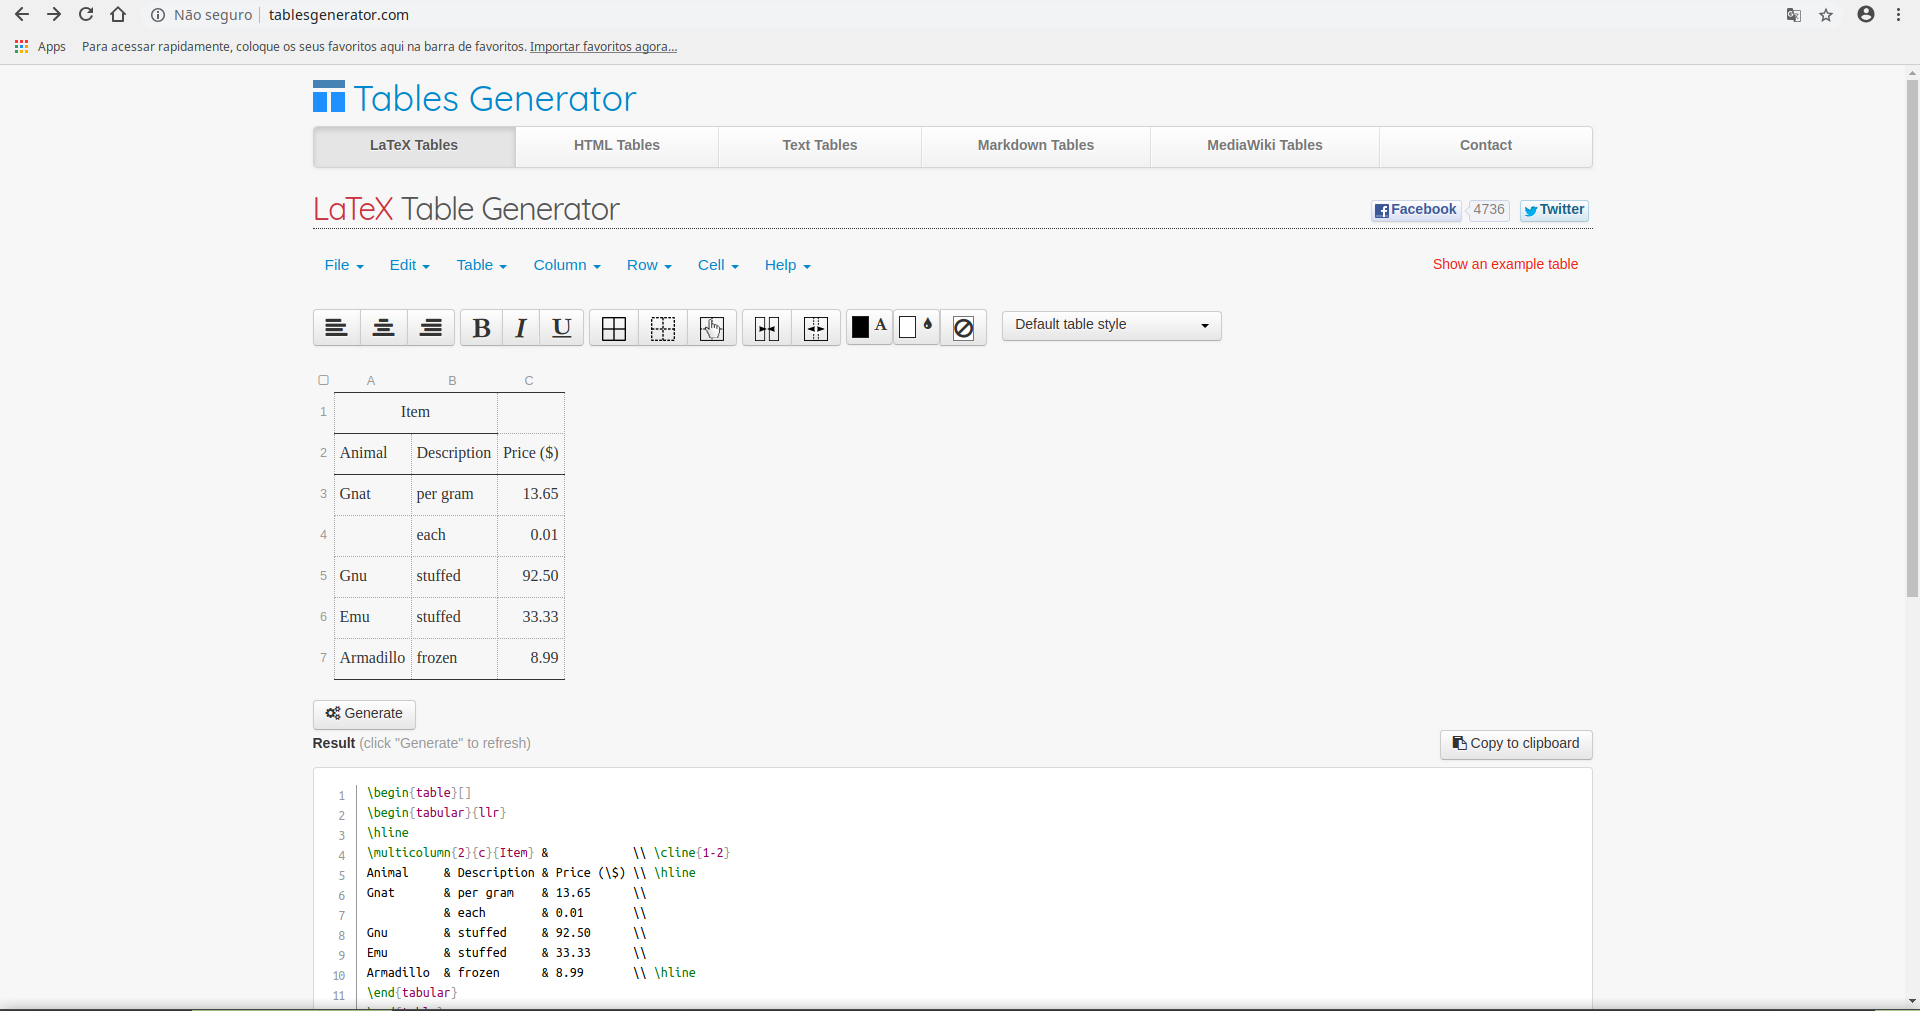
\includegraphics[scale=0.1]{ca.png}
			\end{figure}
			
			Neste gerador de tabelas, basta digitar a conteúdo desejado que ele gera o código correspondente em latex.
		
			
	\section{Pacotes}
		O LaTeX define um conjunto básico de macros para edição de textos. Caso o usuário queira usar alguma função mais complexa o LaTeX permite que ele inclua arquivos com novos macros. Esses arquivos são chamados de pacotes. Existem pacotes para escrever colorido, para incluir figuras, incluir pseudo-código etc. O usuário pode até criar seu próprio pacote. Para incluir um pacote no texto basta digitar a linha:
	
		\begin{figure}[h]
			\centering
			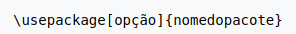
\includegraphics[scale=0.6]{pa.png}
		\end{figure}	
	
		\subsection{aa}
		
		\subsection{aastex}
			Seguindo o exemplo do pacote anterior, o AASTeX foi desenvolvido pela American Astronomical Society (AAS) para auxiliar os autores na preparação de artigos que serão submetidos ao jornal. O pacote foi feito para uso em LaTeX2e e pode ser baixado no link\\ \texttt{https://journals.aas.org/aastex-package-for-manuscript-preparation/}.
			
			Uma vez que o arquivo for baixado, você pode usar o pacote por meio da linha \texttt{$\backslash$documentclass[aastex62]}. Assim, o documento que for digitado seguirá os padrões da AAS.
			
			Entre as funcionalidades do AASTeX, é possível destacar os modelos de tabela que são oferecidos. O pacote usa um ambiente chamado \textit{deluxetable}, fortemente indicado para a construção de tabelas longas. O usuário pode escolher entre usar o modelo padrão do LaTeX e o modelo deluxe do AASTeX. Veja o \textit{deluxetable} em aplicação no seguinte exemplo:
			
			\begin{figure}[h]
				\begin{center}
					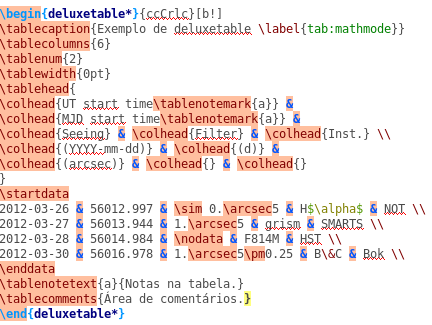
\includegraphics[scale=0.6]{tabelaAASTEX.png}
				\end{center}
			\end{figure}
		
			Assim como a table padrão do LaTeX, o deluxetable guia-se pela definição de "c", "l" e "r" para organizar o posicionamento das colunas. Entretanto, se o usuário estiver utilizando o AASTeX e definir o posicionamento com letras maiúsculas (como ele faz na terceira coluna), o modo Matemática é ativado automaticamente, dispensando assim o uso dos \$s no código. O resultado do código acima é:
			
			\begin{figure}[h]
				\begin{center}
					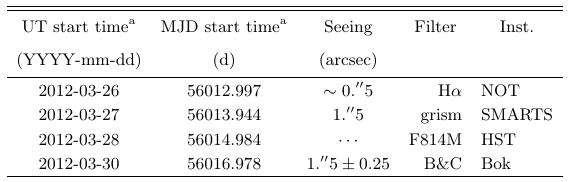
\includegraphics[scale=0.4]{rtabelaAASTEX.png}
				\end{center}
			\end{figure}
			
		
		\subsection{amsart}
			O pacote amsart é amplamente utilizado para publicações da American Mathematical Society, garantindo que o documento editado seguirá os padrões estabelecidos pelo jornal. Na maioria das versões de LaTeX, o pacote já está incluso e pode ser utilizado por meio da linha\\
			\texttt{$\backslash$documentclass[]$\{$amsart$\}$}\\
			Contudo, o pacote pode ser baixado por meio do link \texttt{https://ctan.org/pkg/amsart}, onde o arquivo contém diversos exemplos de como o pacote deve ser utilizado.
		
		\subsection{amscd}
			O pacote amscd, por sua vez, é utilizado para a criação de diagramas comutativos. O pacote, também desenvolvido pela AMS, possui a limitação de oferecer apenas diagramas retangulares, não tendo a capacidade de gerar setas diagonais ou funções mais exóticas.
			
			Para utilizar esse pacote, o usuário deve inserir a linha \texttt{$\backslash$usepackage$\{amscd\}$} e, caso seja necessário, o download do pacote pode ser feito por meio do link \texttt{https://ctan.org/pkg/amscd}. A seguir, um exemplo do código de um diagrama comutativo e seu resultado.
			
			\begin{figure}[h]
				\begin{center}
					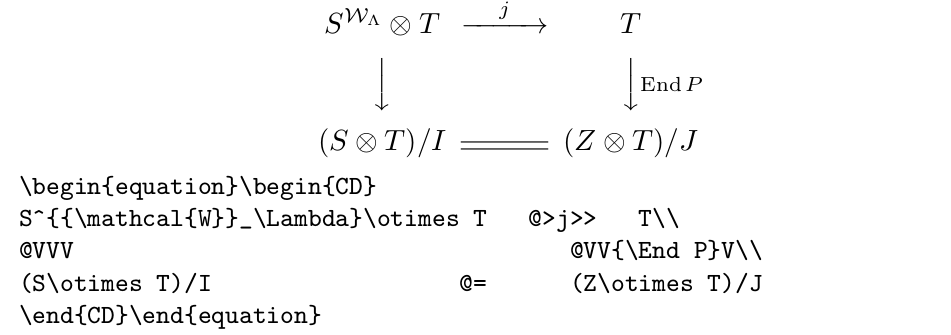
\includegraphics[scale=0.4]{amscd.png}
				\end{center}
			\end{figure}
			
		
		\subsection{amsfonts}
			Voltado para um leque de caracteres matemáticos, o pacote amsfonts carrega diversas variações de fontes já existentes (letras gregas e símbolos matemáticos subscritos), além de incluir novos caracteres (novos símbolos matemáticos e letras Fraktur).
			
			O pacote pode ser incluído através da linha \texttt{$\backslash$usepackage$\{amsfonts\}$} e pode ser baixado, junto com um manual de uso, através do link \texttt{https://ctan.org/pkg/amsfonts}.
		
		\subsection{amsmath}
		
		
		\subsection{amssymb}
		
		\subsection{amsthm}
		
		\subsection{array}
		
		\subsection{article}
		
		\subsection{babel}
		
		\subsection{beamer}
		
		\subsection{biblatex}
		
		\subsection{bm}
		
		\subsection{booktabs}
		
		\subsection{color}
			
		\subsection{dcolumn}
		
		\subsection{enumitem}
		
		\subsection{epsf}
		
		\subsection{espfig}
		
		\subsection{fancyhdr}
		
		\subsection{geometry}
		
		\subsection{graphics}
		
		\subsection{graphicx}
		
		\subsection{hyperref}
			O pacote hyperref fornece ao LaTeX a capacidade de criar hyperlinks dentro do documento. Ele funciona com \textit{pdflatex} e também com o padrão "latex" usado com \textit{dvips} e \textit{ghostscript} ou \textit{dvipdfm} para construir um arquivo PDF. Se você carregá-lo, você terá a possibilidade de incluir links externos interativos e todas as suas referências internas serão transformadas em hiperlinks. O compilador \textit{pdflatex} torna possível criar arquivos PDF diretamente da fonte LaTeX, e o PDF suporta mais recursos que o DVI. Em particular, o PDF suporta hiperlinks. Além disso, o PDF pode conter outras informações sobre um documento, como o título, o autor, etc., que podem ser editadas usando o mesmo pacote.\\
			O uso básico com as configurações padrão é simples. Basta carregar o pacote no preâmbulo:
			\begin{figure}[h]
				\centering
				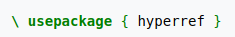
\includegraphics[scale=0.6]{caa.png}
			\end{figure}
		
			Isso automaticamente transformará todas as suas referências internas em hiperlinks. Isso não afetará a maneira de escrever seus documentos: basta continuar usando o padrão $\backslash$label- $\backslash$refsistema (discutido no capítulo sobre etiquetas e referências cruzadas); com hyperref essas "conexões" se tornarão links e você poderá clicar neles para ser redirecionado para a página correta. Além disso, o índice, a lista de figuras $\backslash$ tabelas e o índice serão também feitos de hiperlinks. Os hiperlinks não serão exibidos se você estiver trabalhando no modo de rascunho.\\
			Exemplo 1:
			\begin{figure}[h]
				\centering
				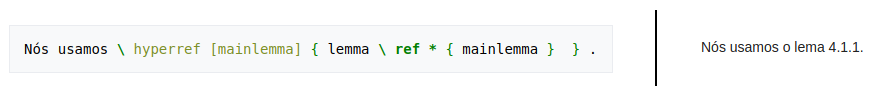
\includegraphics[scale=0.5]{ref.png}
			\end{figure}
		
			Exemplo 2: 
			\begin{figure}[h]
				\centering
				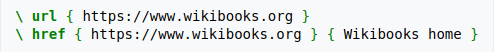
\includegraphics[scale=0.6]{si.png}
			\end{figure}
		
			Exemplo 3: ARRUMAR AQUI
			
			
			
			
			
			
			%ERRO DE IMAGEM
			
			
			
			
			
			
			
			
			\begin{figure}[h]
				\centering
				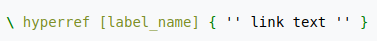
\includegraphics[scale=0.6]{f.png}
			\end{figure}
		
		\subsection{latexsym}
			O pacote latexsym fornece 11 símbolos matemáticos que foram originalmente definidos no LaTeX2.09, mas não são mais definidos no Esquema de Seleção de Novas Fontes. 
			Esses símbolos também são fornecidos pelos pacotes amsfonts e amssymb. Como o SWP e o SW chamam o pacote amsfonts automaticamente, normalmente você não precisa adicionar o pacote latexsym ao seu documento para obter os símbolos. Nenhuma opção de pacote está disponível. O pacote latexsym está instalado no diretório base TCITeX / TeX / LaTeX /. O site para download é:\\
			https://www.mackichan.com/index.html?techtalk/500.htm~mainFram\\ e o arquivo deve estar armazenado na mesma pasta dos arquivos LaTeX.
		
		\subsection{listings}
			Usando as listagens de pacotes, você pode adicionar texto não formatado como faria com, mas seu objetivo principal é incluir o código-fonte de qualquer linguagem de programação em seu documento. Para usar o pacote, você precisa:\\
			\begin{center}
				$\backslash$usepackage \{{ listagens }\}
			\end{center}
			O pacote de listagens suporta o destaque de todos os idiomas mais comuns e é altamente personalizável. Se você quiser apenas escrever código em seu documento, o pacote fornece o ambiente lstlisting:\\
			Exemplo 1:
			\begin{figure}[h]
				\centering
				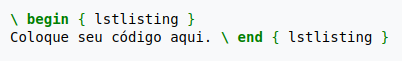
\includegraphics[scale=0.6]{dd.png}
			\end{figure}\\
			Exemplo 2:
			\begin{figure}[h]
				\centering
				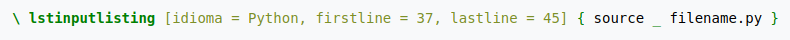
\includegraphics[scale=0.6]{py.png}
			\end{figure}\\
			Exemplo 3:
			\begin{figure}[h]
				\centering
				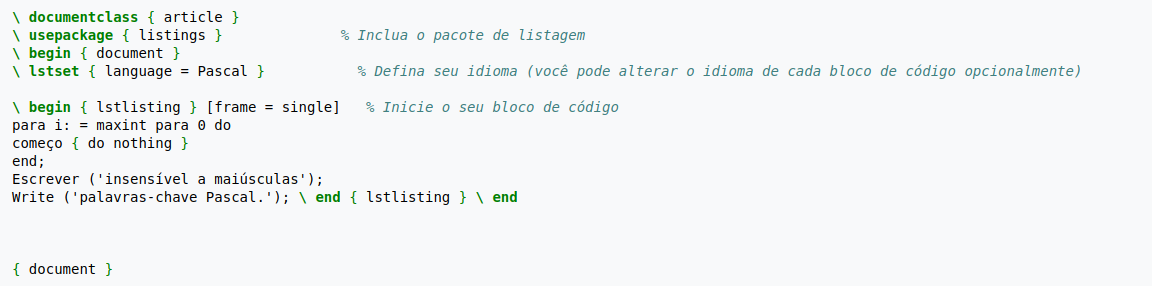
\includegraphics[scale=0.4]{do.png}
			\end{figure}
		
		\subsection{microtype}
			Este pacote faz pequenos ajustes na distribuição, tamanho e forma das letras em cada linha de maneira que o texto esteja alinhado à esquerda e à direita simultaneamente sem introduzir espaçamento excessivo entre as palavras e com uma apresentação agradável, facilitando a leitura. Para usar o pacote, você precisa:\\
			\begin{center}
				$\backslash$usepackage\{{microtype}\}
			\end{center}
			Exemplo 1:\\
			\begin{center}
				$\backslash$usepackage[tracking=alltext,letterspace=-40]{microtype}
			\end{center}
			Exemplo 2:\\
			\begin{center}
				$\backslash$usepackage[protrusion=allmath,tracking=smallcaps]\{{microtype}\}
			\end{center}
		
		\subsection{multicol}
			Se você está escrevendo um texto em uma única coluna e quer que parte dele apareça em mais colunas, você
			pode fazer isso usando o pacote \textit{multicol}. Para isso basta colocar no preâmbulo o comando:\\
			\begin{center}
				$\backslash$usepackage\{{multicol}\}
			\end{center}
			Com esse pacote podemos escrever textos não só em 2 colunas, como também em 3, 4, . . . Par isso escreva
			o texto que irá aparecer em várias colunas de $\backslash$begin \{{multicols}\}\{{n}\} e $\backslash$end\{{multicols}\}, e no lugar de n coloque o número de colunas que você quer. Por exemplo, digitando o texto:
			\begin{figure}[h]
				\centering
				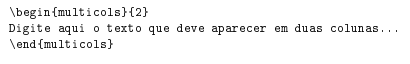
\includegraphics[scale=0.8]{co.png}
			\end{figure}
		
			e o texto vai aparecer assim:
		
			\begin{figure}[h]
				\centering
				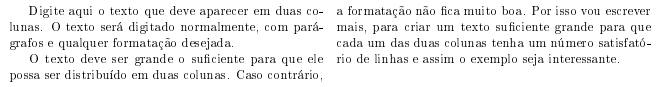
\includegraphics[scale=0.7]{exp.png}
			\end{figure}
			Tudo que for digitado depois de $\backslash$end\{{multicols}\} volta a ser apresentado em uma única coluna.
		
		\subsection{revtex/revtex4}
			REVTeX é um conjunto de pacotes para serem usados com LaTeX2e. A primeira versão foi lançada em 1986. A quarta versão, REVTeX 4, em 2001. A
			versão atual é a REVTeX 4.1. Estes pacotes são destinados à redação de artigos para a submissão
			nas revistas da APS e AIP.\\
			Para realizar a instalação basta seguir o passo a passo:\\
			\begin{itemize}
			
				\item Baixe revtex4-1.zip do seguinte endereço: https://authors.aps.org/revtex4/
				\item Extraia revtex4-1.zip e dentro desta pasta abra o terminal
				\item No terminal copie e cole:  “sudo unzip revtex4-1-tds.zip -d /etc/texmf”
				\item Para incluir o pacote  revtex4-1 em seu documento latex adicione: $\backslash$documentclass [preprintnumbers,amsmath,amssymb,pre,floatfix]\{{revtex4-1}\}
			
			\end{itemize}
			Exemplo:
			
			
			
			
			
			%ERRO NA IMAGEM
			
			
			
			
			
			
			
			
			\begin{figure}[h]
				\centering
				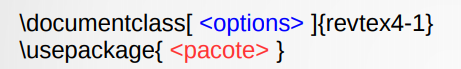
\includegraphics[scale=0.6]{re.png}
			\end{figure}
		
		
		\subsection{times}
			O pacote times já é obsoleto devido ao bug do escalamento das fontes. Em vez do times, use a combinação de mathptmx, helvet, e courier ($\backslash$usepackage\{{math\\ptmx,courier}\} $\backslash$usepackage[scaled=.92]{helvet}) em vez do times para mapear fontes para ser compatíveis com o times: Adobe Times para roman (fonte de espaçamento variável para corpo do texto) e  math (fórmula), Helvetica para Sans Serif (fontes sem a serifa), Courier para typewriter (fontes mono espaçados para códigos). Note que a fonte typewriter é mais fino que demais fontes e as fontes e símbolos adicionais tais como fontes do AMS, Black board bold fonts, etc, não serão oferecidos e eles podem ficar como no original (normalmente, compatível com a fonte Computer Modern).  Para ter fontes tudo compatíveis com times, opte pelo pacote txfonts.\\
			Para usar o pacote, você precisa:\\
		
			\begin{center}
				$\backslash$usepackage\{{times}\}
			\end{center}
		
		
	
\end{document}